\chapter{Burgers' equation}
The Reynolds number of a flow measures the relative importance of inertia and viscous forces. If it is below the critical Reynolds number, the flow is smooth and regular, it is a laminar flow. If the Reynolds number is above the critical Reynolds, the flow becomes random and chaotic. It becomes a turbulent flow \cite{Versteeg2007}.

Unfortunately, turbulence is the usual state of motion of the fluids, except at very low Reynolds numbers. When the Reynolds number is high, the inertial forces lead to instabilities. In this regime, the properties of the flow are irregular, with three-dimensional fluctuations \cite{CTTCb}. These turbulent motions are rotating swirls named eddies.

There are different scales of eddies in a turbulent flow \cite{Pope2000}. The large ones control the transport and mixing in the flow, and are influenced by the geometry. On the other hand, small eddies depend on the energy that receive from the large scales and on the viscosity. Large eddies are unstable and tend to break, transferring their energy to smaller eddies. These smaller eddies also break, transferring their spectral energy to even smaller eddies, and so on. This process of energy transfer to smaller scales is called energy cascade.

As a consequence, depending on their size, eddies have different energy. Typically, energy is injected in the larger scales. This is called the production range. Then, in the inertial range, there is a transfer of energy from larger scales to smaller ones. In this range, the motion of the eddies is determined by the inertial effects, with viscosity still being negligible. And, finally, in even smaller scales, the energy is dissipated due to the viscous effects. This process is represented in figure \ref{energylength}.

\begin{figure}
	\centering
	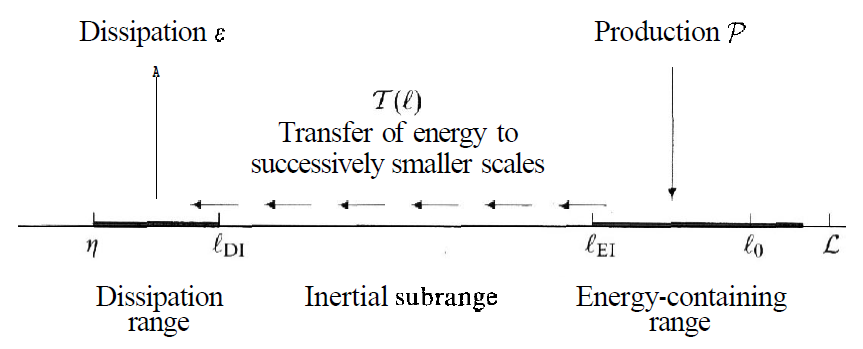
\includegraphics[scale=0.6]{Burgers/energylength}
	\caption[Schematic diagram of the energy cascade as a function of the size of the eddies]{Schematic diagram of the energy cascade as a function of the size of the eddies. Extracted from \cite{Pope2000}}
	\label{energylength}
\end{figure}

In conclusion, turbulence is very complex. It requires to model different scales, and to take into account non-linear effects. Navier-Stokes equations can describe this non-linearity of turbulence, but their numerical simulation is difficult. Moreover, since the scale of the eddies can become really small, the number of control volumes required in the simulation would be very high, and the resulting code would be computationally expensive. To simplify the calculations, Burgers proposed a one-dimensional model for turbulence: the Burgers' equation.

\section{Burgulence}
Burgers' equation, also known as Burgulence, is a one dimensional approach to the momentum equation in an incompressible flow. It is the simplest equation that combines non-linearity and dissipation \cite{Johnson2016}. Its non-dimensional expression is:
\begin{equation}
\frac{\partial u}{\partial t}+u\frac{\partial u}{\partial x}=\frac{1}{Re}\frac{\partial^{2}u}{\partial x^{2}}+f
\end{equation}
where $u$ is the velocity in the studied dimension, $Re$ the Reynolds number and $f$ the source term.

Since the equation is one-dimensional, the continuity equation is removed. The pressure gradient is also removed because it depends on the continuity equation.

\section{Fourier space}
The easiest way to solve the equation is to solve it in Fourier space. The basic approach of this space is that any function can be represented as a sum of sinus and cosines known as Fourier series in the following way:
\begin{equation}
u\left(x\right)=\sum_{k=-\infty}^{k=+\infty}û_{k}e^{ikx}
\end{equation}
where $e^{ikx}=\cos\left(kx\right)+i\sin\left(kx\right)$, with $k=2\pi/l$ being the wavenumber, a parameter that depends on the length of the eddies.

Nonetheless, in a numerical calculation, it is impossible to have an infinite number of terms, it is necessary to have a finite number. Fortunately, in spectral methods the biggest amount of information is in the lowest frequencies, which means that it is not necessary to have a huge amount of terms in order to have a proper solution of the equation. Taking this into account, the functions that are represented in the Fourier space become a sum of a finite number of sinus and cosines:
\begin{equation}
u\left(x\right)=\sum_{k=-N}^{k=+N}û_{k}e^{ikx}
\end{equation}
Using this expression, the Burgers' equation can be transformed into the Fourier space. However, the derivatives have to be calculated. Applying the derivative to the Fourier function definition:
\begin{equation}
\frac{\partial u}{\partial x}=\frac{\partial}{\partial x}\sum_{k=-N}^{k=+N}û_{k}e^{ikx}=\sum_{k=-N}^{k=+N}û_{k}\frac{\partial e^{ikx}}{\partial x}=\sum_{k=-N}^{k=+N}û_{k}\left(ik\right)e^{ikx}
\end{equation}

The same procedure is applied to the second derivative in order to obtain the diffusive term:
\begin{multline}
\frac{\partial^{2}u}{\partial x^{2}}=\frac{\partial}{\partial x}\left(\frac{\partial u}{\partial x}\right)=\frac{\partial}{\partial x}\sum_{k=-N}^{k=+N}û_{k}\left(ik\right)e^{ikx}=\sum_{k=-N}^{k=+N}û_{k}\left(ik\right)\frac{\partial e^{ikx}}{\partial x}= \\
\sum_{k=-N}^{k=+N}û_{k}\left(ik\right)^{2}e^{ikx}=\sum_{k=-N}^{k=+N}\left(-k^{2}û_{k}\right)e^{ikx}
\end{multline}
The transient \ref{TransientTerm} and forcing \ref{ForcingTerm} terms are straightforward:
\begin{equation}
\frac{\partial u}{\partial t}=\frac{\partial}{\partial t}\sum_{k=-N}^{k=+N}û_{k}e^{ikx}
\label{TransientTerm}
\end{equation}
\begin{equation}
f=\sum_{k=-N}^{k=+N}F_{k}e^{ikx}
\label{ForcingTerm}
\end{equation}

On the other hand, the convective term is more complicated. This non-linear term is a multiplication of the function $u$ and its derivative, and when it is transformed into Fourier space there are some things that need to be taken into account. The terms in question are:
\begin{equation}
\frac{\partial u}{\partial x}=\sum_{q=-N}^{q=+N}iqû_{q}e^{iqx}
\end{equation}
\begin{equation}
u=\sum_{p=-N}^{p=+N}û_{p}e^{ipx}
\end{equation}
As it is noted, the variable k has been renamed in both terms in order to avoid confusions when the expressions are multiplied to obtain the convective term. It is finally calculated as:
\begin{equation}
u\frac{\partial u}{\partial x}=\sum_{p,q}û_{p}iqû_{q}e^{i\left(ptq\right)x}
\end{equation}
Taking all these expressions, integrating them into the Burgers equation and applying the Fourier transform, the final expression is:
\begin{equation}
\frac{\partial û_{k}}{\partial t}+\sum_{p+q=k}û_{p}iqû_{q}=-\frac{k^{2}}{Re}û_{k}+F_{k}
\end{equation}
for $k=1,\dots, N$; and where $û_{k}\in\mathbb{C}$.

One of the main advantages of spectral methods is that all the modes can be solved separately. However, due to the convective term, there is still a sum of terms in the equation, named triadic interactions. This summation can be easily interpreted with figure \ref{TriadicFigure}.
\begin{figure}
	\centering
	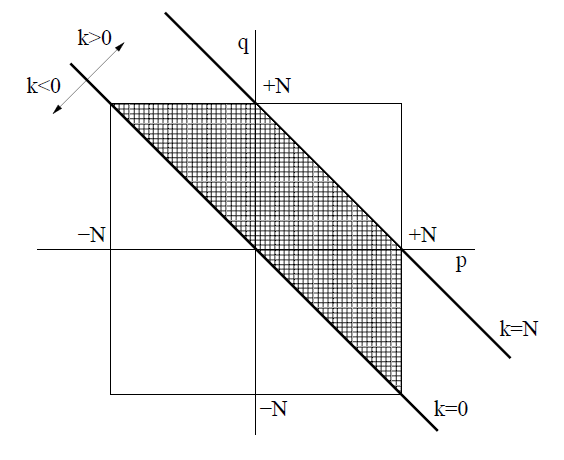
\includegraphics[scale=0.7]{Burgers/Burger}
	\caption[Representation of all the possible interactions between the modes in the convective term]{Representation of all the possible interactions between the modes in the convective term. Extracted from \cite{CTTC2014}}
	\label{TriadicFigure}
\end{figure}
In Fourier space $\bar{û}_{-k}=û_{k}$, so only the positive modes need to be solved. Moreover, since the Fourier series are truncated for $k\leq|N|$, the only possible interactions are those of $p+q\leq N$. Therefore, only the interactions between the lines $k=0$ and $k=+N$ have to be considered in the computation of the convective term.

\section{Discretization}
In order to solve the equation it is necessary to discretize it over time. The time-integration scheme used is the fully explicit one:
\begin{equation}
\frac{û_{k}^{n+1}-û_{k}^{n}}{\Delta t}+\sum_{p+q=k}û_{q}iqû_{q}=-\frac{k^{2}}{Re}û_{k}+F_{k}
\label{DiscretizedBurgers}
\end{equation}
However, the time step needs to be small enough to guarantee good results. A CFL-like condition is imposed:
\begin{equation}
\Delta t\leq C_{1}\frac{Re}{N^{2}}
\end{equation}

The calculation of the kinetic energy as a function of the wavenumber is simply done as:
\begin{equation}
E_{k}=|û_{k}|^{2}
\end{equation}

\subsection{Direct Numerical Simulation}
The direct application of the equation \ref{DiscretizedBurgers} to obtain $û_{k}^{n+1}$ is called Direct Numerical Simulation (DNS). It is the simplest method, and it does not use any model approximation. However, in order to provide accurate results, several modes of the equation have to be solved.

\subsection{Large-Eddy Simulation}
A method that can improve the calculations of the DNS is the Large-Eddy Simulation (LES). Like DNS, it starts with a one-dimensional equation in which the unknown is not the velocity but its average.
\begin{equation}
\frac{\partial\bar{u}}{\partial t}+\bar{u}\frac{\partial\bar{u}}{\partial x}=\frac{1}{Re}\frac{\partial^{2}\bar{u}}{\partial x^{2}}+f-\frac{\partial}{\partial x}\tau\left(u\right)
\end{equation}
where
\begin{equation}
\tau\left(u\right)=\bar{u^{2}}-\bar{u}^{2}
\end{equation}
In the model proposed by Smagorinsky, this subfilter tensor is modeled using a viscosity called the eddy-viscosity \cite{CTTC2014}:
\begin{equation}
\tau\left(u\right)\approx\nu_{t}\frac{\partial\bar{u}}{\partial x}
\end{equation}
The Smagorinsky model also proposes an expression for $\nu_{t}$, but it cannot be applied in Fourier space. To do so, a spectral viscosity model is used:
\begin{equation}
\nu_{t}\left(k/k_{N}\right)=\nu_{t}^{+\infty}\left(\frac{E_{k_{N}}}{k_{N}}\right)^{1/2}\nu_{t}^{*}\left(\frac{k}{k_N}\right)
\end{equation}
with
\begin{equation}
\nu_{t}^{+\infty}=0.31\frac{5-m}{m+1}\sqrt{3-m}C_{K}^{-3/2}
\end{equation}
\begin{equation}
\nu_{t}^{*}\left(\frac{k}{k_{N}}\right)=1+34.5e^{-3.03\left(k_N/k\right)}
\end{equation}
where $m$ is the slope of the energy spectrum, $E_{k_{N}}$ is the energy at the truncated frequency $k_{N}$, and $C_{K}$ is the Kolmogorov constant. With the results obtained with the DNS, it can be deduced that $m\approx2$. And for the value of the Kolomogorov constant, it is known that for the one-dimensional Burgers' equation it is $C_{K}\approx0.4523$.

\section{Algorithm}
A scheme of the algorithm used to solve the Burgers' equation is displayed below. The problem ends when the simulation reaches a steady state.
\begin{figure}[H]
	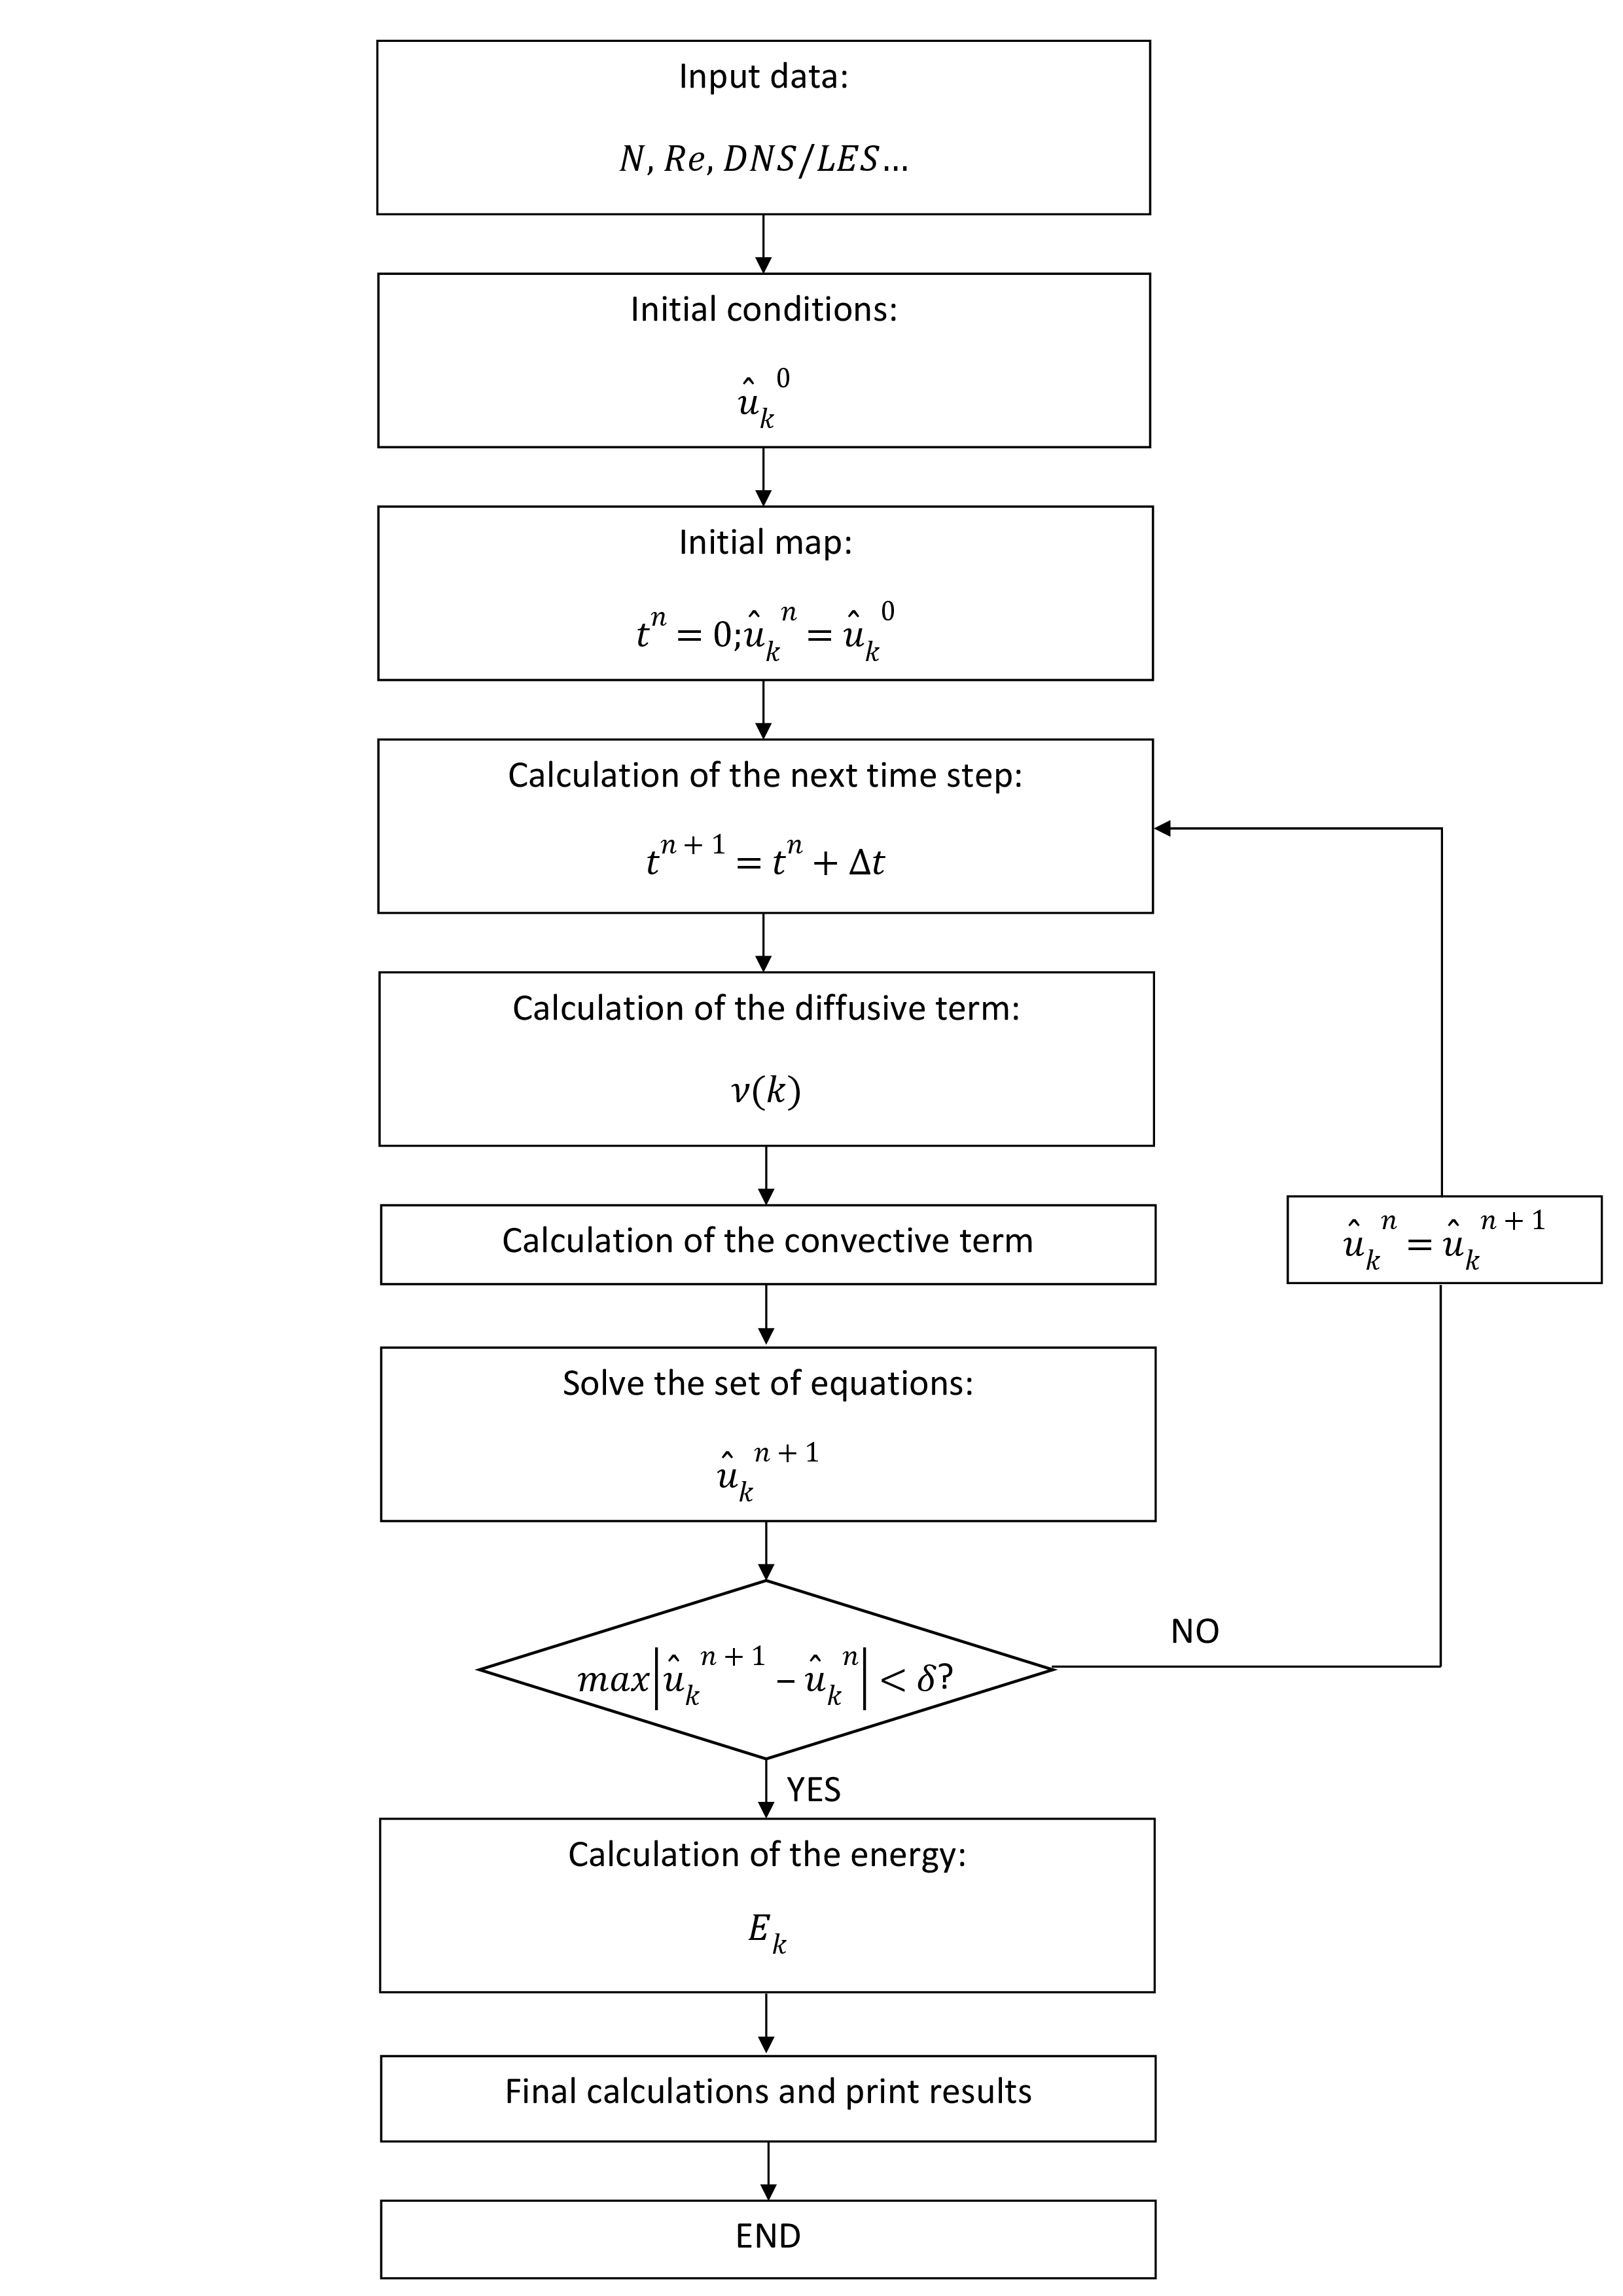
\includegraphics[scale=0.15]{Burgers/Doc5}
\end{figure}

\section{Results}
In order to obtain the energy cascade, the Burgers' equation has been solved using DNS and LES. The following results are studied for $Re=40$, taking as initial conditions:
\begin{equation}
û_{k}=k^{-1}
\end{equation}
Figure \ref{BurgersResults} represents the energy cascade in a logarithmic plot. As the wavenumber $k$ increases (the length of the eddies decreases), the kinetic energy decreases. For bigger eddies, inertia makes the flow more chaotic and the energy is higher, but as their length decreases, the viscosity becomes more important and the energy is reduced.
\begin{figure}[h]
	\centering
	\chapter{Burgers' equation}
Burgers' equation, also known as Burgulence, is a one dimensional approach to the Navier-Stokes equations in an incompressible flow. Taking the dimensionless expressions that describe an incompressible flow:

%https://books.google.es/books?id=TQfYCwAAQBAJ&printsec=frontcover&hl=es#v=onepage&q&f=false 
%pag 4-33

\begin{equation}
\frac{\partial\vec{v}}{\partial t}+\left(\vec{v}\cdot\nabla\right)\vec{v}=\frac{1}{Re}\nabla^{2}\vec{v}-\nabla p
\end{equation}
\begin{equation}
\nabla\cdot\vec{v}=0
\label{ContinuityIncomp}
\end{equation}
And writing their one-dimensional form, the Burgers equation is easily obtained:
\begin{equation}
\frac{\partial u}{\partial t}+u\frac{\partial u}{\partial x}=\frac{1}{Re}\frac{\partial^{2}u}{\partial x^{2}}+f
\end{equation}
where $u$ is the velocity in the studied dimension and $f$ the source term.

Since the equation is one-dimensional, the continuity equation \ref{ContinuityIncomp} is removed. The pressure gradient is also removed because it depends on the continuity equation.

\section{Fourier space}
The easiest way to solve the equation is to solve it in Fourier space. The basic approach of this space is that any function can be represented as a sum of sinus and cosines known as Fourier series in the following way:
\begin{equation}
u\left(x\right)=\sum_{k=-\infty}^{k=+\infty}û_{k}e^{ikx}
\end{equation}
where $e^{ikx}=\cos\left(kx\right)+i\sin\left(kx\right)$.

Nonetheless, in a numerical calculation, it is impossible to have an infinite number of terms, it is necessary to have a finite number. This is not a problem, because in spectral methods, the biggest amount of information is in the lowest frequencies, which means that it is not necessary to have a huge amount of terms in order to have a proper solution of the equation. Taking this into account, the functions that are represented in the Fourier space become a sum of a finite number of sinus and cosines:
\begin{equation}
u\left(x\right)=\sum_{k=-N}^{k=+N}û_{k}e^{ikx}
\end{equation}
Using this expression, the Burgers' equation can be transformed into the Fourier space. However, the derivatives have to be calculated. Applying the derivative to the Fourier function definition:
\begin{equation}
\frac{\partial u}{\partial x}=\frac{\partial}{\partial x}\sum_{k=-N}^{k=+N}û_{k}e^{ikx}=\sum_{k=-N}^{k=+N}û_{k}\frac{\partial e^{ikx}}{\partial x}=\sum_{k=-N}^{k=+N}û_{k}\left(ik\right)e^{ikx}
\end{equation}

The same procedure is applied to the second derivative in order to obtain the diffusive term:
\begin{multline}
\frac{\partial^{2}u}{\partial x^{2}}=\frac{\partial}{\partial x}\left(\frac{\partial u}{\partial x}\right)=\frac{\partial}{\partial x}\sum_{k=-N}^{k=+N}û_{k}\left(ik\right)e^{ikx}=\sum_{k=-N}^{k=+N}û_{k}\left(ik\right)\frac{\partial e^{ikx}}{\partial x}= \\
\sum_{k=-N}^{k=+N}û_{k}\left(ik\right)^{2}e^{ikx}=\sum_{k=-N}^{k=+N}\left(-k^{2}û_{k}\right)e^{ikx}
\end{multline}
The transient \ref{TransientTerm} and forcing \ref{ForcingTerm} terms are straightforward:
\begin{equation}
\frac{\partial u}{\partial t}=\frac{\partial}{\partial t}\sum_{k=-N}^{k=+N}û_{k}e^{ikx}
\label{TransientTerm}
\end{equation}
\begin{equation}
f=\sum_{k=-N}^{k=+N}F_{k}e^{ikx}
\label{ForcingTerm}
\end{equation}

On the other, the convective term is more complicated. This non-linear term is a multiplication of the function u and its derivative, and when this term is transformed into Fourier space there are some things that need to be taken into account. The terms in question are:
\begin{equation}
\frac{\partial u}{\partial x}=\sum_{q=-N}^{q=+N}iqû_{q}e^{iqx}
\end{equation}
\begin{equation}
u=\sum_{p=-N}^{p=+N}û_{p}e^{ipx}
\end{equation}
As it is noted, the variable k has been renamed in both terms in order to avoid confusions when the expressions are multiplied to obtain the convective term. It is finally calculated as:
\begin{equation}
u\frac{\partial u}{\partial x}=\sum_{p,q}û_{p}iqû_{q}e^{i\left(ptq\right)x}
\end{equation}
Taking all these expressions, integrating them into the Burgers equation and applying the Fourier transform, the final expression is:
\begin{equation}
\frac{\partial û_{k}}{\partial t}+\sum_{p+q=k}û_{p}iqû_{q}=-\frac{k^{2}}{Re}û_{k}+F_{k}
\end{equation}
for $k=1,\dots, N$; and where $û_{k}\in\mathbb{C}$.

As it can be seen, one of the main advantages of spectral methods is that all the modes can be solved separately. However, due to the convective term, there is still a sum of terms in the equation, which can be named triadic interactions. This summation can be easily interpreted with figure \ref{TriadicFigure}.
\begin{figure}
	\centering
	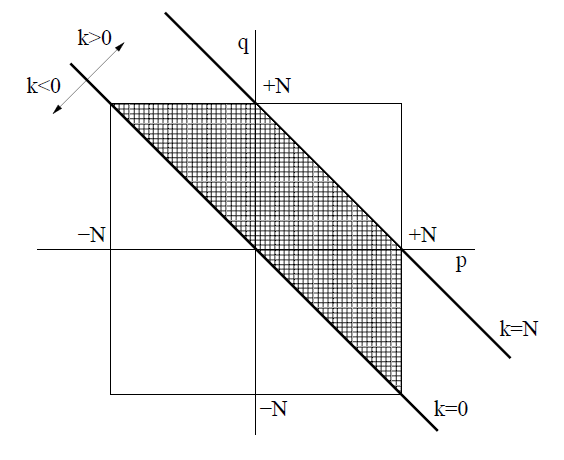
\includegraphics[scale=0.7]{Burgers/Burger}
	\caption[Representation of all the possible interactions between the modes in the convective term]{Representation of all the possible interactions between the modes in the convective term. Extracted from \cite{CTTC2014}}
	\label{TriadicFigure}
\end{figure}
In Fourier space $\bar{û}_{-k}=û_{k}$, so only the positive modes need to be solved. Moreover, since the Fourier series are truncated for $k\leq|N|$, the only possible interactions are those of $p+q\leq N$. Therefore, only the interactions between the lines $k=0$ and $k=+N$ have to be considered in the computation of the convective term.

\section{Discretization}
In order to solve the equation it is necessary to discretize it over time. The time-integration scheme used is the fully explicit one:
\begin{equation}
\frac{û_{k}^{n+1}-û_{k}^{n}}{\Delta t}+\sum_{p+q=k}û_{q}iqû_{q}=-\frac{k^{2}}{Re}û_{k}+F_{k}
\end{equation}
However, the time step needs to be small enough to guarantee good results. A CFL-like condition is imposed:
\begin{equation}
\Delta t\leq C_{1}\frac{Re}{N^{2}}
\end{equation}

\subsection{Large-Eddy Simulation}
The method proposed in the previous lines is called Direct Numerical Simulation (DNS), and it does not provide as good results as other methods based on some turbulence models. A method that can improve the calculations is the Large-Eddy Simulation (LES). Like the DNS, it starts with a one-dimensional equation in which the unknown is not the velocity but its average.
\begin{equation}
\frac{\partial\bar{u}}{\partial t}+\bar{u}\frac{\partial\bar{u}}{\partial x}=\frac{1}{Re}\frac{\partial^{2}\bar{u}}{\partial x^{2}}+f-\frac{\partial}{\partial x}\tau\left(u\right)
\end{equation}
where
\begin{equation}
\tau\left(u\right)=\bar{u^{2}}-\bar{u}^{2}
\end{equation}
In the Smagorinsky model, this subfilter tensor is modeled using a viscosity called the eddy-viscosity:
\begin{equation}
\tau\left(u\right)\approx\nu_{t}\frac{\partial\bar{u}}{\partial x}
\end{equation}
Smagorinsky also obtained an expression for $\nu_{t}$, but it cannot be applied in Fourier space. To do so, a spectral viscosity model is used:
\begin{equation}
\nu_{t}\left(k/k_{N}\right)=\nu_{t}^{+\infty}\left(\frac{E_{k_{N}}}{k_{N}}\right)^{1/2}\nu_{t}^{*}\left(\frac{k}{k_N}\right)
\end{equation}
where
\begin{equation}
\nu_{t}^{+\infty}=0.31\frac{5-m}{m+1}\sqrt{3-m}C_{K}^{-3/2}
\end{equation}
\begin{equation}
\nu_{t}^{*}\left(\frac{k}{k_{N}}\right)=1+34.5e^{-3.03\left(k_N/k\right)}
\end{equation}
where $m$ is the slope of the energy spectrum, $E_{k_{N}}$ is the energy at the truncated frequency $k_{N}$, and $C_{K}$ is the Kolmogorov constant. With the results obtained with the DNS, it can be deduced that $m=2$ approximately. And for the value of the Kolomogorov constant, it is known that for the one-dimensional Burgers' equation it is $C_{K}\approx0.4523$.

\section{Results}
\begin{figure}[h]
	\centering
	\chapter{Burgers' equation}
Burgers' equation, also known as Burgulence, is a one dimensional approach to the Navier-Stokes equations in an incompressible flow. Taking the dimensionless expressions that describe an incompressible flow:

%https://books.google.es/books?id=TQfYCwAAQBAJ&printsec=frontcover&hl=es#v=onepage&q&f=false 
%pag 4-33

\begin{equation}
\frac{\partial\vec{v}}{\partial t}+\left(\vec{v}\cdot\nabla\right)\vec{v}=\frac{1}{Re}\nabla^{2}\vec{v}-\nabla p
\end{equation}
\begin{equation}
\nabla\cdot\vec{v}=0
\label{ContinuityIncomp}
\end{equation}
And writing their one-dimensional form, the Burgers equation is easily obtained:
\begin{equation}
\frac{\partial u}{\partial t}+u\frac{\partial u}{\partial x}=\frac{1}{Re}\frac{\partial^{2}u}{\partial x^{2}}+f
\end{equation}
where $u$ is the velocity in the studied dimension and $f$ the source term.

Since the equation is one-dimensional, the continuity equation \ref{ContinuityIncomp} is removed. The pressure gradient is also removed because it depends on the continuity equation.

\section{Fourier space}
The easiest way to solve the equation is to solve it in Fourier space. The basic approach of this space is that any function can be represented as a sum of sinus and cosines known as Fourier series in the following way:
\begin{equation}
u\left(x\right)=\sum_{k=-\infty}^{k=+\infty}û_{k}e^{ikx}
\end{equation}
where $e^{ikx}=\cos\left(kx\right)+i\sin\left(kx\right)$.

Nonetheless, in a numerical calculation, it is impossible to have an infinite number of terms, it is necessary to have a finite number. This is not a problem, because in spectral methods, the biggest amount of information is in the lowest frequencies, which means that it is not necessary to have a huge amount of terms in order to have a proper solution of the equation. Taking this into account, the functions that are represented in the Fourier space become a sum of a finite number of sinus and cosines:
\begin{equation}
u\left(x\right)=\sum_{k=-N}^{k=+N}û_{k}e^{ikx}
\end{equation}
Using this expression, the Burgers' equation can be transformed into the Fourier space. However, the derivatives have to be calculated. Applying the derivative to the Fourier function definition:
\begin{equation}
\frac{\partial u}{\partial x}=\frac{\partial}{\partial x}\sum_{k=-N}^{k=+N}û_{k}e^{ikx}=\sum_{k=-N}^{k=+N}û_{k}\frac{\partial e^{ikx}}{\partial x}=\sum_{k=-N}^{k=+N}û_{k}\left(ik\right)e^{ikx}
\end{equation}

The same procedure is applied to the second derivative in order to obtain the diffusive term:
\begin{multline}
\frac{\partial^{2}u}{\partial x^{2}}=\frac{\partial}{\partial x}\left(\frac{\partial u}{\partial x}\right)=\frac{\partial}{\partial x}\sum_{k=-N}^{k=+N}û_{k}\left(ik\right)e^{ikx}=\sum_{k=-N}^{k=+N}û_{k}\left(ik\right)\frac{\partial e^{ikx}}{\partial x}= \\
\sum_{k=-N}^{k=+N}û_{k}\left(ik\right)^{2}e^{ikx}=\sum_{k=-N}^{k=+N}\left(-k^{2}û_{k}\right)e^{ikx}
\end{multline}
The transient \ref{TransientTerm} and forcing \ref{ForcingTerm} terms are straightforward:
\begin{equation}
\frac{\partial u}{\partial t}=\frac{\partial}{\partial t}\sum_{k=-N}^{k=+N}û_{k}e^{ikx}
\label{TransientTerm}
\end{equation}
\begin{equation}
f=\sum_{k=-N}^{k=+N}F_{k}e^{ikx}
\label{ForcingTerm}
\end{equation}

On the other, the convective term is more complicated. This non-linear term is a multiplication of the function u and its derivative, and when this term is transformed into Fourier space there are some things that need to be taken into account. The terms in question are:
\begin{equation}
\frac{\partial u}{\partial x}=\sum_{q=-N}^{q=+N}iqû_{q}e^{iqx}
\end{equation}
\begin{equation}
u=\sum_{p=-N}^{p=+N}û_{p}e^{ipx}
\end{equation}
As it is noted, the variable k has been renamed in both terms in order to avoid confusions when the expressions are multiplied to obtain the convective term. It is finally calculated as:
\begin{equation}
u\frac{\partial u}{\partial x}=\sum_{p,q}û_{p}iqû_{q}e^{i\left(ptq\right)x}
\end{equation}
Taking all these expressions, integrating them into the Burgers equation and applying the Fourier transform, the final expression is:
\begin{equation}
\frac{\partial û_{k}}{\partial t}+\sum_{p+q=k}û_{p}iqû_{q}=-\frac{k^{2}}{Re}û_{k}+F_{k}
\end{equation}
for $k=1,\dots, N$; and where $û_{k}\in\mathbb{C}$.

As it can be seen, one of the main advantages of spectral methods is that all the modes can be solved separately. However, due to the convective term, there is still a sum of terms in the equation, which can be named triadic interactions. This summation can be easily interpreted with figure \ref{TriadicFigure}.
\begin{figure}
	\centering
	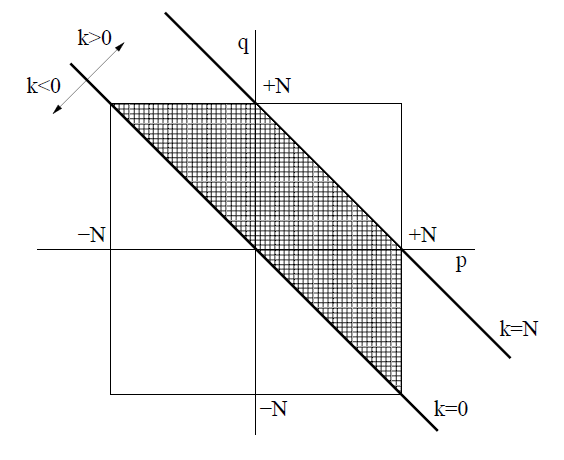
\includegraphics[scale=0.7]{Burgers/Burger}
	\caption[Representation of all the possible interactions between the modes in the convective term]{Representation of all the possible interactions between the modes in the convective term. Extracted from \cite{CTTC2014}}
	\label{TriadicFigure}
\end{figure}
In Fourier space $\bar{û}_{-k}=û_{k}$, so only the positive modes need to be solved. Moreover, since the Fourier series are truncated for $k\leq|N|$, the only possible interactions are those of $p+q\leq N$. Therefore, only the interactions between the lines $k=0$ and $k=+N$ have to be considered in the computation of the convective term.

\section{Discretization}
In order to solve the equation it is necessary to discretize it over time. The time-integration scheme used is the fully explicit one:
\begin{equation}
\frac{û_{k}^{n+1}-û_{k}^{n}}{\Delta t}+\sum_{p+q=k}û_{q}iqû_{q}=-\frac{k^{2}}{Re}û_{k}+F_{k}
\end{equation}
However, the time step needs to be small enough to guarantee good results. A CFL-like condition is imposed:
\begin{equation}
\Delta t\leq C_{1}\frac{Re}{N^{2}}
\end{equation}

\subsection{Large-Eddy Simulation}
The method proposed in the previous lines is called Direct Numerical Simulation (DNS), and it does not provide as good results as other methods based on some turbulence models. A method that can improve the calculations is the Large-Eddy Simulation (LES). Like the DNS, it starts with a one-dimensional equation in which the unknown is not the velocity but its average.
\begin{equation}
\frac{\partial\bar{u}}{\partial t}+\bar{u}\frac{\partial\bar{u}}{\partial x}=\frac{1}{Re}\frac{\partial^{2}\bar{u}}{\partial x^{2}}+f-\frac{\partial}{\partial x}\tau\left(u\right)
\end{equation}
where
\begin{equation}
\tau\left(u\right)=\bar{u^{2}}-\bar{u}^{2}
\end{equation}
In the Smagorinsky model, this subfilter tensor is modeled using a viscosity called the eddy-viscosity:
\begin{equation}
\tau\left(u\right)\approx\nu_{t}\frac{\partial\bar{u}}{\partial x}
\end{equation}
Smagorinsky also obtained an expression for $\nu_{t}$, but it cannot be applied in Fourier space. To do so, a spectral viscosity model is used:
\begin{equation}
\nu_{t}\left(k/k_{N}\right)=\nu_{t}^{+\infty}\left(\frac{E_{k_{N}}}{k_{N}}\right)^{1/2}\nu_{t}^{*}\left(\frac{k}{k_N}\right)
\end{equation}
where
\begin{equation}
\nu_{t}^{+\infty}=0.31\frac{5-m}{m+1}\sqrt{3-m}C_{K}^{-3/2}
\end{equation}
\begin{equation}
\nu_{t}^{*}\left(\frac{k}{k_{N}}\right)=1+34.5e^{-3.03\left(k_N/k\right)}
\end{equation}
where $m$ is the slope of the energy spectrum, $E_{k_{N}}$ is the energy at the truncated frequency $k_{N}$, and $C_{K}$ is the Kolmogorov constant. With the results obtained with the DNS, it can be deduced that $m=2$ approximately. And for the value of the Kolomogorov constant, it is known that for the one-dimensional Burgers' equation it is $C_{K}\approx0.4523$.

\section{Results}
\begin{figure}[h]
	\centering
	\chapter{Burgers' equation}
Burgers' equation, also known as Burgulence, is a one dimensional approach to the Navier-Stokes equations in an incompressible flow. Taking the dimensionless expressions that describe an incompressible flow:

%https://books.google.es/books?id=TQfYCwAAQBAJ&printsec=frontcover&hl=es#v=onepage&q&f=false 
%pag 4-33

\begin{equation}
\frac{\partial\vec{v}}{\partial t}+\left(\vec{v}\cdot\nabla\right)\vec{v}=\frac{1}{Re}\nabla^{2}\vec{v}-\nabla p
\end{equation}
\begin{equation}
\nabla\cdot\vec{v}=0
\label{ContinuityIncomp}
\end{equation}
And writing their one-dimensional form, the Burgers equation is easily obtained:
\begin{equation}
\frac{\partial u}{\partial t}+u\frac{\partial u}{\partial x}=\frac{1}{Re}\frac{\partial^{2}u}{\partial x^{2}}+f
\end{equation}
where $u$ is the velocity in the studied dimension and $f$ the source term.

Since the equation is one-dimensional, the continuity equation \ref{ContinuityIncomp} is removed. The pressure gradient is also removed because it depends on the continuity equation.

\section{Fourier space}
The easiest way to solve the equation is to solve it in Fourier space. The basic approach of this space is that any function can be represented as a sum of sinus and cosines known as Fourier series in the following way:
\begin{equation}
u\left(x\right)=\sum_{k=-\infty}^{k=+\infty}û_{k}e^{ikx}
\end{equation}
where $e^{ikx}=\cos\left(kx\right)+i\sin\left(kx\right)$.

Nonetheless, in a numerical calculation, it is impossible to have an infinite number of terms, it is necessary to have a finite number. This is not a problem, because in spectral methods, the biggest amount of information is in the lowest frequencies, which means that it is not necessary to have a huge amount of terms in order to have a proper solution of the equation. Taking this into account, the functions that are represented in the Fourier space become a sum of a finite number of sinus and cosines:
\begin{equation}
u\left(x\right)=\sum_{k=-N}^{k=+N}û_{k}e^{ikx}
\end{equation}
Using this expression, the Burgers' equation can be transformed into the Fourier space. However, the derivatives have to be calculated. Applying the derivative to the Fourier function definition:
\begin{equation}
\frac{\partial u}{\partial x}=\frac{\partial}{\partial x}\sum_{k=-N}^{k=+N}û_{k}e^{ikx}=\sum_{k=-N}^{k=+N}û_{k}\frac{\partial e^{ikx}}{\partial x}=\sum_{k=-N}^{k=+N}û_{k}\left(ik\right)e^{ikx}
\end{equation}

The same procedure is applied to the second derivative in order to obtain the diffusive term:
\begin{multline}
\frac{\partial^{2}u}{\partial x^{2}}=\frac{\partial}{\partial x}\left(\frac{\partial u}{\partial x}\right)=\frac{\partial}{\partial x}\sum_{k=-N}^{k=+N}û_{k}\left(ik\right)e^{ikx}=\sum_{k=-N}^{k=+N}û_{k}\left(ik\right)\frac{\partial e^{ikx}}{\partial x}= \\
\sum_{k=-N}^{k=+N}û_{k}\left(ik\right)^{2}e^{ikx}=\sum_{k=-N}^{k=+N}\left(-k^{2}û_{k}\right)e^{ikx}
\end{multline}
The transient \ref{TransientTerm} and forcing \ref{ForcingTerm} terms are straightforward:
\begin{equation}
\frac{\partial u}{\partial t}=\frac{\partial}{\partial t}\sum_{k=-N}^{k=+N}û_{k}e^{ikx}
\label{TransientTerm}
\end{equation}
\begin{equation}
f=\sum_{k=-N}^{k=+N}F_{k}e^{ikx}
\label{ForcingTerm}
\end{equation}

On the other, the convective term is more complicated. This non-linear term is a multiplication of the function u and its derivative, and when this term is transformed into Fourier space there are some things that need to be taken into account. The terms in question are:
\begin{equation}
\frac{\partial u}{\partial x}=\sum_{q=-N}^{q=+N}iqû_{q}e^{iqx}
\end{equation}
\begin{equation}
u=\sum_{p=-N}^{p=+N}û_{p}e^{ipx}
\end{equation}
As it is noted, the variable k has been renamed in both terms in order to avoid confusions when the expressions are multiplied to obtain the convective term. It is finally calculated as:
\begin{equation}
u\frac{\partial u}{\partial x}=\sum_{p,q}û_{p}iqû_{q}e^{i\left(ptq\right)x}
\end{equation}
Taking all these expressions, integrating them into the Burgers equation and applying the Fourier transform, the final expression is:
\begin{equation}
\frac{\partial û_{k}}{\partial t}+\sum_{p+q=k}û_{p}iqû_{q}=-\frac{k^{2}}{Re}û_{k}+F_{k}
\end{equation}
for $k=1,\dots, N$; and where $û_{k}\in\mathbb{C}$.

As it can be seen, one of the main advantages of spectral methods is that all the modes can be solved separately. However, due to the convective term, there is still a sum of terms in the equation, which can be named triadic interactions. This summation can be easily interpreted with figure \ref{TriadicFigure}.
\begin{figure}
	\centering
	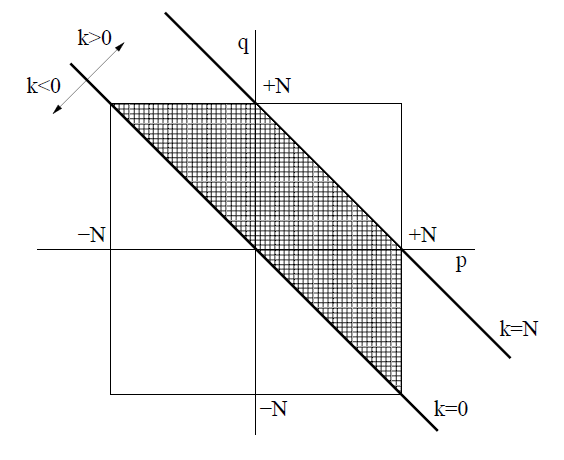
\includegraphics[scale=0.7]{Burgers/Burger}
	\caption[Representation of all the possible interactions between the modes in the convective term]{Representation of all the possible interactions between the modes in the convective term. Extracted from \cite{CTTC2014}}
	\label{TriadicFigure}
\end{figure}
In Fourier space $\bar{û}_{-k}=û_{k}$, so only the positive modes need to be solved. Moreover, since the Fourier series are truncated for $k\leq|N|$, the only possible interactions are those of $p+q\leq N$. Therefore, only the interactions between the lines $k=0$ and $k=+N$ have to be considered in the computation of the convective term.

\section{Discretization}
In order to solve the equation it is necessary to discretize it over time. The time-integration scheme used is the fully explicit one:
\begin{equation}
\frac{û_{k}^{n+1}-û_{k}^{n}}{\Delta t}+\sum_{p+q=k}û_{q}iqû_{q}=-\frac{k^{2}}{Re}û_{k}+F_{k}
\end{equation}
However, the time step needs to be small enough to guarantee good results. A CFL-like condition is imposed:
\begin{equation}
\Delta t\leq C_{1}\frac{Re}{N^{2}}
\end{equation}

\subsection{Large-Eddy Simulation}
The method proposed in the previous lines is called Direct Numerical Simulation (DNS), and it does not provide as good results as other methods based on some turbulence models. A method that can improve the calculations is the Large-Eddy Simulation (LES). Like the DNS, it starts with a one-dimensional equation in which the unknown is not the velocity but its average.
\begin{equation}
\frac{\partial\bar{u}}{\partial t}+\bar{u}\frac{\partial\bar{u}}{\partial x}=\frac{1}{Re}\frac{\partial^{2}\bar{u}}{\partial x^{2}}+f-\frac{\partial}{\partial x}\tau\left(u\right)
\end{equation}
where
\begin{equation}
\tau\left(u\right)=\bar{u^{2}}-\bar{u}^{2}
\end{equation}
In the Smagorinsky model, this subfilter tensor is modeled using a viscosity called the eddy-viscosity:
\begin{equation}
\tau\left(u\right)\approx\nu_{t}\frac{\partial\bar{u}}{\partial x}
\end{equation}
Smagorinsky also obtained an expression for $\nu_{t}$, but it cannot be applied in Fourier space. To do so, a spectral viscosity model is used:
\begin{equation}
\nu_{t}\left(k/k_{N}\right)=\nu_{t}^{+\infty}\left(\frac{E_{k_{N}}}{k_{N}}\right)^{1/2}\nu_{t}^{*}\left(\frac{k}{k_N}\right)
\end{equation}
where
\begin{equation}
\nu_{t}^{+\infty}=0.31\frac{5-m}{m+1}\sqrt{3-m}C_{K}^{-3/2}
\end{equation}
\begin{equation}
\nu_{t}^{*}\left(\frac{k}{k_{N}}\right)=1+34.5e^{-3.03\left(k_N/k\right)}
\end{equation}
where $m$ is the slope of the energy spectrum, $E_{k_{N}}$ is the energy at the truncated frequency $k_{N}$, and $C_{K}$ is the Kolmogorov constant. With the results obtained with the DNS, it can be deduced that $m=2$ approximately. And for the value of the Kolomogorov constant, it is known that for the one-dimensional Burgers' equation it is $C_{K}\approx0.4523$.

\section{Results}
\begin{figure}[h]
	\centering
	\input{Burgers/Burgers}
	\caption{Energy spectrum of the steady-state solution of the Burgers' equation}
\end{figure}
	\caption{Energy spectrum of the steady-state solution of the Burgers' equation}
\end{figure}
	\caption{Energy spectrum of the steady-state solution of the Burgers' equation}
\end{figure}
	\caption{Energy spectrum of the steady-state solution of the Burgers' equation}
	\label{BurgersResults}
\end{figure}

As it can be seen, different simulations have been computed. In the case of the DNS, the results are obtained using 20 modes and 100 nodes. For $N=20$, the solution is not really precise, some more nodes have to be computed. However, the results for $N=100$ are more accurate.

In the case of LES, even with less nodes, the results are better. For $C_{K}=0.4523$, the solution is very similar to that obtained in the case of $N=100$ using DNS for low wavenumbers. With the same number of nodes, the results are better, even though the calculations are more complicated.